\documentclass[12pt]{beamer}
\usepackage{breqn}
\usepackage[brazilian,hyperpageref]{backref}
\usepackage[num]{abntex2cite}		% Citações padrão ABNT
\usepackage[utf8]{inputenc}
\usepackage[portuguese]{babel}
\usepackage{colortbl}
\usepackage{color}
\usepackage{amsmath}
\usepackage{url}
\usepackage{hyperref}
\usepackage{beamerthemeshadow}
%\usepackage{lstlisting}
\usepackage{listings}

\graphicspath{{./images/}}
\citebrackets[]

\setbeamertemplate{bibliography item}{\insertbiblabel}
\setbeamertemplate{caption}[numbered]

\renewcommand{\backrefpagesname}{Citado na(s) página(s):~}
% Texto padrão antes do número das páginas
\renewcommand{\backref}{}
% Define os textos da citação
\renewcommand*{\backrefalt}[4]{}
    %\ifcase #1 %
        %Nenhuma citação no texto.%
    %\or
        %Citado na página #2.%
    %\else
        %Citado #1 vezes nas páginas #2.%
    %\fi}%

\beamertemplatenavigationsymbolsempty% tira os elementos de navegação da parte de baixo
%\setbeamertemplate{footline}{}%remove o autor e o título da parte de baixo

\addtobeamertemplate{navigation symbols}{}{%
    \usebeamerfont{footline}%
    \usebeamercolor[black]{footline}%
    \hspace{1em}%
    Página~\insertframenumber~de~\inserttotalframenumber
}

\usetheme{Frankfurt}
\usecolortheme{orchid}

\author{Victor Emanuel Almeida}
\title{Conceitos básicos de C++ para maratona de programação}
\date{\today}
\institute{UNIOESTE}
\logo{
\includegraphics[height=1cm]{logo_unioeste.jpg}}

\definecolor{dkgreen}{rgb}{0,0.6,0}
\definecolor{gray}{rgb}{0.5,0.5,0.5}
\definecolor{mauve}{rgb}{0.58,0,0.82}
\definecolor{laranja_claro}{rgb}{1,0.9,0.5}
\definecolor{laranja_escuro}{rgb}{1,0.5,0.2}
\definecolor{azul_claro}{rgb}{0.5,0.9,1}

\lstset{frame=tb,
    language=C,
    frame=tb,
    aboveskip=3mm,
    belowskip=3mm,
    showstringspaces=false,
    columns=flexible,
    basicstyle={\small\ttfamily},
    numbers=left,
    numberstyle=\tiny\color{gray},
    keywordstyle=\color{blue},
    commentstyle=\color{dkgreen},
    stringstyle=\color{mauve},
    breaklines=true,
    breakatwhitespace=true,
    xleftmargin=.05\textwidth,
    xrightmargin=.05\textwidth,
    tabsize=4,
}

\begin{document}
\frame{\titlepage}

\begin{frame}
    \frametitle{Conteúdo}
    \tableofcontents
\end{frame}

\section{Características C++}\label{Características C++}
\begin{frame}[allowframebreaks]
    \frametitle{Conceitos}
    \begin{figure}[!htb]
        \centering
        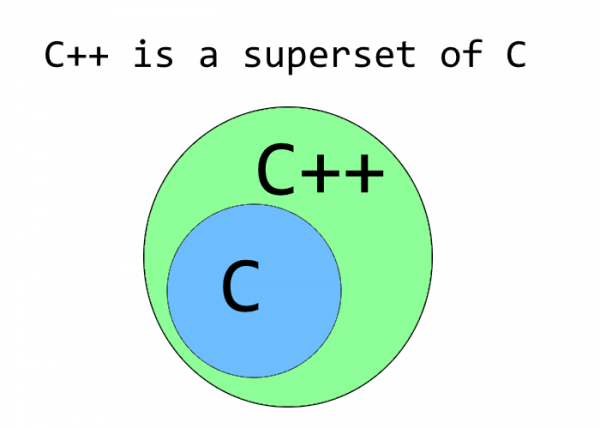
\includegraphics[width=.7\textwidth]{superset}
        \caption{\label{fig:superset}Diagrama de Venn C/C++}
    \end{figure}
    \framebreak
    \begin{figure}[!htb]
        \centering
        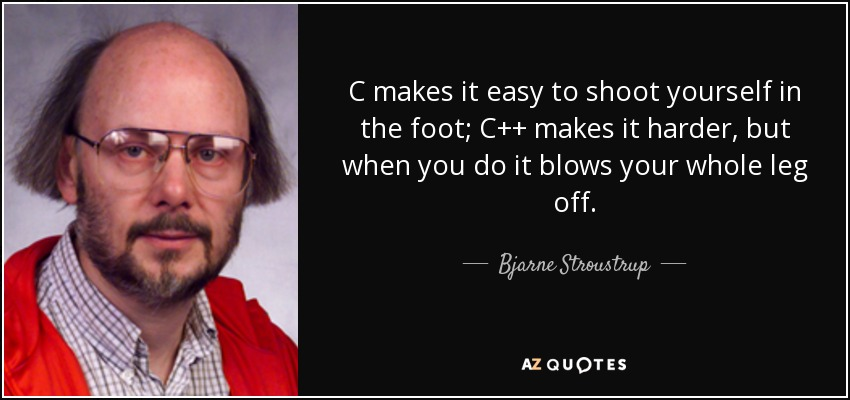
\includegraphics[width=\textwidth]{frase_c++}
    \end{figure}
    \framebreak
    \begin{itemize}
        \item Linguagem compilada (g++);
        \item Fortemente tipada\cite{slides_clp_2};
        \item Multiparadigma: Imperativa e orientada a objetos\cite{slides_clp_2};
        \item Linguagem complexa com muitas instruções e palavras reservadas\cite{slides_clp_2}.
    \end{itemize}
\end{frame}

\begin{frame}
    \frametitle{Vantagens do C++ sobre o C}
    \begin{itemize}
        \item Orientação a objetos;
        \item Entrada e saída de dados;
        \item Sobrecarga de operadores;
        \item Referências;
        \item Alocação de memória e smart pointers;
        \item Bibliotecas padrão com algoritmos e estruturas de dados.
    \end{itemize}
\end{frame}

\section{Ola Mundo}\label{Ola Mundo}
\begin{frame}[t,fragile]{\insertsectionhead}
    \frametitle{Exemplo de Ola Mundo Simples}
    \begin{lstlisting}
#include <iostream>
using namespace std;
int main () {
    cout << "Ola Mundo\n";
    return 0;
}
    \end{lstlisting}
\end{frame}

\section{Sobrecarga de operador}\label{Sobrecarga de operador}
\begin{frame}
    \frametitle{Explicando o $<<$}
\end{frame}

\section{Dicas c++ Maratona}\label{Dicas c++ Maratona}
\begin{frame}[t,fragile]{\insertsectionhead}
    \frametitle{Exemplo de Ola Mundo Maratona}
    \begin{center}
    \begin{lstlisting}
#include <bits/stdc++.h>
using namespace std;
int main () {
    // desabilita a sincronizacao entre as streams do c com do c++
    // retire se for usar printf e scanf
    ios_base::sync_with_stdio(false);
    // desabilita o flush automatico do buffer
    // retire caso use um cout sem fim de linha e logo em seguida cin
    cin.tie(0);
    cout << "Ola Mundo\n";
    return 0;
}
    \end{lstlisting}
    \end{center}
\end{frame}

\section{Estruturas de dados STL}
\begin{frame}[allowframebreaks]
    \frametitle{Sequenciais}

    Vetores:
    Tem uma ``api'' idêntica a vetores do C com acesso de um elemento específico, ``vetor[i] = valor;''

    \begin{itemize}
        \item\textbf{array$<$T, size$>$}: Vetor do tipo T de tamanho size definido em tempo de compilação;
        \item\textbf{vector$<$T$>$}: Vetor do tipo T de tamanho variável;
        \item \textbf{deque$<$T$>$}: Fila duplamente encadeada do tipo T, funciona como o vector porém as ações de inserir e remover são um pouco mais eficientes;
    \end{itemize}

    \framebreak

    Listas encadeadas: Não possui acesso a um elemento específico
    \begin{itemize}
        \item\textbf{forward\_list$<$T$>$}: Lista encadeada do tipo T, so pode ser percorrida do começo para o fim;
        \item\textbf{list$<$T$>$}: Lista duplamente encadeada do tipo T, pode ser percorrida dos dois lados;
    \end{itemize}
\end{frame}

\begin{frame}
    \frametitle{Interfaces FIFO e LIFO}

    Interfaces que por padrão utilizam estruturas como deque e list internamente:

    \begin{itemize}
        \item\textbf{stack$<$T$>$}: Pilha do tipo T, funciona como uma pilha de pratos, o último a entrar é o primeiro a sair (\textit{LIFO, Last In First Out});
        \item\textbf{queue$<$T$>$}: Fila do tipo T, funciona como uma fila de banco, o primeiro a entrar é o primeiro a sair (\textit{FIFO, First In First Out});
    \end{itemize}

\end{frame}

\begin{frame}[allowframebreaks]
    \frametitle{Associativas}

    Implementam estruturas que permitem buscar um elemento de forma eficiente $O(\log(N))$ normalmente utilizando árvores como a rubro-negra ou tabelas hash.
    \begin{itemize}
        \item\textbf{set$<$T$>$}: Conjunto do tipo T, não permite elementos repetidos, é uma árvore rubro-negra;
        \item\textbf{map$<$K, V$>$}: Mapeia a chave do tipo K para um valor do tipo V, não permite chaves repetidas, é uma árvore rubro-negra;
    \end{itemize}

    \framebreak
    Modificadores de estruturas associativas (multi e unordered):
    \begin{itemize}
        \item\textbf{multi}: Permite elementos repetidos, no caso da map chaves repetidas;
        \item\textbf{unordered}: Elementos não são alocados de maneira sequencial na estrutura;
    \end{itemize}

    \framebreak
    \begin{itemize}
        \item\textbf{set}: Árvore rubro-negra;
        \item\textbf{multiset}: Árvore rubro-negra;
        \item\textbf{unordered\_set}: Tabela hash;
        \item\textbf{unordered\_multiset}: Tabela hash;

        \item\textbf{map}: Árvore rubro-negra;
        \item\textbf{multimap}: Árvore rubro-negra;
        \item\textbf{unordered\_map}: Tabela hash;
        \item\textbf{unordered\_multimap}: Tabela hash;
    \end{itemize}

\end{frame}

\begin{frame}
    \frametitle{Exemplo}

\end{frame}

\section{Exercício}\label{Exercício}
\begin{frame}
    \frametitle{Enunciado}

    You are given a list of n integers,
    and your task is to calculate the number
    of distinct values in the list.

\end{frame}

\section{Referências}\label{Referências}
\begin{frame}[allowframebreaks]
    \frametitle{Referências}
    \bibliography{ref}
\end{frame}

\end{document}
